\documentclass[conference,twocolumn]{IEEEtran}

% Packages
\usepackage[utf8]{inputenc}
\usepackage[T1]{fontenc}
\usepackage{graphicx}
\usepackage{amsmath,amssymb}
\usepackage{hyperref}
\usepackage{booktabs}
\usepackage{enumitem}
\usepackage{listings}
\usepackage{xcolor}
\usepackage{float}
\usepackage{caption}
\usepackage{algorithm}
\usepackage{algpseudocode}
\usepackage{cite}
\usepackage{url}

% Code listing style
\lstdefinestyle{python}{
    language=Python,
    basicstyle=\ttfamily\footnotesize,
    keywordstyle=\color{blue},
    stringstyle=\color{red},
    commentstyle=\color{green!60!black},
    frame=single,
    breaklines=true,
    tabsize=4,
    showstringspaces=false
}

% Hyperref setup
\hypersetup{
    colorlinks=true,
    linkcolor=blue,
    urlcolor=blue,
    citecolor=blue
}

\begin{document}

% Title
\title{Performance Modeling for Real-World Cloud Message Queue Systems: An Enhanced Analytical and Simulation Framework}

\author{
\IEEEauthorblockN{Himanshu Jain}
\IEEEauthorblockA{Department of Software Engineering\\
San Jose State University\\
San Jose, CA, USA\\
himanshu.jain@sjsu.edu}
\and
\IEEEauthorblockN{Bhuvana Komati}
\IEEEauthorblockA{Department of Software Engineering\\
San Jose State University\\
San Jose, CA, USA\\
bhuvana.komati@sjsu.edu}
}

\maketitle

% Abstract
\begin{abstract}
Cloud message brokers are critical infrastructure components enabling asynchronous communication in distributed systems. This paper extends the foundational work of Li et al. (2015) to address limitations in modeling real-world cloud message queue performance. While the base paper assumes exponential service times (M/M/N model), our research demonstrates that real cloud workloads exhibit heavy-tailed (Pareto) distributions where standard models underestimate P99 latency by up to \textbf{45\%}. We developed an enhanced analytical and simulation framework using Python/SimPy incorporating heavy-tailed service time distributions, explicit threading architectures, and distributed consistency protocols (Two-Phase Commit, Raft Consensus). Our key findings reveal that heavy-tailed distributions cause P99/mean latency ratios exceeding 36x, traffic amplification validates to 0.2\% error, and Two-Phase Commit adds 36\% service time overhead. The framework includes a full-stack implementation with React frontend and FastAPI backend for interactive capacity planning.
\end{abstract}

\begin{IEEEkeywords}
Queueing Theory, Message Brokers, Heavy-Tailed Distributions, Pareto Distribution, Two-Phase Commit, Cloud Computing, P99 Latency
\end{IEEEkeywords}

% Introduction
\section{Introduction}

Cloud message brokers serve as the backbone of modern distributed systems, enabling reliable asynchronous communication between services. Systems like AWS SQS, RabbitMQ, Apache Kafka, and Azure Queue Storage handle billions of messages daily, making accurate performance modeling critical for capacity planning, SLA compliance, and cost optimization.

Traditional queueing models (M/M/N) assume exponential service times with convenient mathematical properties. However, real-world observations from Google \cite{dean2013}, Amazon \cite{decandia2007}, and Netflix show that cloud workloads exhibit heavy-tailed behavior where the P99/mean latency ratio can exceed 36x compared to the 4.6x predicted by exponential models.

This paper makes the following contributions:
\begin{enumerate}[leftmargin=*]
    \item Reproduction and validation of Li et al.'s M/M/N tandem queue results
    \item Extension to support heavy-tailed (Pareto) service distributions
    \item Quantification of the ``reality gap'' between theory and practice
    \item Implementation of distributed consistency protocols (2PC, Raft)
    \item Interactive visualization tools for engineering analysis
\end{enumerate}

% Base Paper Overview
\section{Related Work}

\subsection{Base Paper: Li et al. (2015)}

Li et al. \cite{li2015} proposed a tandem queue model for cloud message brokers using Colored Petri Nets. Their key contribution was the traffic inflation formula:

\begin{equation}
\Lambda_2 = \frac{\lambda}{1-p}
\end{equation}

where $\lambda$ is the arrival rate and $p$ is the failure probability causing retransmissions. The paper validated results against M/M/N analytical solutions but assumed exponential service times.

\subsection{Heavy-Tailed Distributions}

Dean and Barroso \cite{dean2013} documented that P99 latencies dominate user experience in large-scale systems. The Pareto distribution captures this behavior:

\begin{equation}
P(X > x) = \left(\frac{x_m}{x}\right)^\alpha \quad \text{for } x \geq x_m
\end{equation}

When $\alpha \leq 2$, variance becomes infinite, making traditional confidence intervals unreliable.

% System Model
\section{System Model}

\subsection{Tandem Queue Architecture}

Our system models a two-stage message broker where messages flow from producers through Stage 1 (sender queue) to Stage 2 (receiver queue). Failed messages are retransmitted, creating traffic amplification.

\begin{table}[h]
\centering
\caption{System Parameters}
\begin{tabular}{lll}
\toprule
\textbf{Parameter} & \textbf{Symbol} & \textbf{Value} \\
\midrule
Arrival rate & $\lambda$ & 80 msg/sec \\
Service rate (Stage 1) & $\mu_1$ & 10 msg/sec \\
Service rate (Stage 2) & $\mu_2$ & 12 msg/sec \\
Servers (Stage 1) & $N_1$ & 10 \\
Servers (Stage 2) & $N_2$ & 8 \\
Failure probability & $p$ & 0.1 \\
\bottomrule
\end{tabular}
\label{tab:params}
\end{table}

\subsection{Mathematical Foundation}

Our framework is built on 15 core equations organized into three categories.

\subsubsection{M/M/N Baseline}

The utilization and Erlang-C formula:

\begin{equation}
\rho = \frac{\lambda}{N \cdot \mu}
\end{equation}

\begin{equation}
C(N, a) = \frac{\frac{a^N}{N!} \cdot \frac{N}{N-a}}{\sum_{k=0}^{N-1}\frac{a^k}{k!} + \frac{a^N}{N!} \cdot \frac{N}{N-a}}
\end{equation}

Mean queue wait time:

\begin{equation}
W_q = \frac{C(N, a)}{\mu \cdot N \cdot (1-\rho)}
\end{equation}

\subsubsection{Heavy-Tailed Extensions}

Pareto probability density function:

\begin{equation}
f(x) = \frac{\alpha \cdot x_m^\alpha}{x^{\alpha+1}} \quad \text{for } x \geq x_m
\end{equation}

Kingman's M/G/N approximation:

\begin{equation}
W_q^{M/G/N} \approx W_q^{M/M/N} \cdot \frac{1 + C_s^2}{2}
\end{equation}

where $C_s^2$ is the squared coefficient of variation.

\subsubsection{P99 Latency}

Standard Gaussian approximation:

\begin{equation}
W_{99} \approx W_{\text{mean}} + 2.33 \cdot \sigma_W
\end{equation}

This fails for heavy tails where:

\begin{equation}
P(W > w) \sim w^{-\alpha}
\end{equation}

% Implementation
\section{Implementation}

\subsection{Technology Stack}

We implemented the framework using:
\begin{itemize}[leftmargin=*]
    \item \textbf{Simulation:} SimPy 4.1.1 (discrete-event)
    \item \textbf{Backend:} FastAPI + Pydantic (REST API)
    \item \textbf{Frontend:} React 18 + TypeScript
    \item \textbf{Analysis:} NumPy + SciPy
\end{itemize}

\subsection{SimPy vs Colored Petri Nets}

We chose SimPy over CPNs for flexibility in implementing custom distributions, easier debugging, and seamless REST API integration.

\begin{lstlisting}[style=python, caption={M/M/N Queue Implementation}]
class MMNQueue:
  def __init__(self, env, n, mu):
    self.servers = simpy.Resource(
      env, capacity=n)
    self.mu = mu
    
  def process(self, msg_id):
    with self.servers.request() as req:
      yield req
      yield self.env.timeout(
        random.expovariate(self.mu))
\end{lstlisting}

\subsection{Distributed Protocols}

We implemented Two-Phase Commit (2PC) and Raft consensus for distributed scenarios:

\begin{algorithm}[h]
\caption{Two-Phase Commit}
\begin{algorithmic}[1]
\Procedure{2PC}{msg, participants}
\State \textbf{Phase 1:} Send PREPARE to all
\If{all vote YES}
    \State \textbf{Phase 2:} Send COMMIT
\Else
    \State Send ABORT
\EndIf
\EndProcedure
\end{algorithmic}
\end{algorithm}

% Results
\section{Experimental Results}

\subsection{Baseline Validation}

Our SimPy implementation matches analytical M/M/N within 2\%:

\begin{table}[h]
\centering
\caption{Baseline Validation Results}
\begin{tabular}{lccc}
\toprule
\textbf{Metric} & \textbf{Analytical} & \textbf{Simulation} & \textbf{Error} \\
\midrule
Mean Wait & 0.0125s & 0.0127s & 1.6\% \\
Queue Length & 1.00 & 0.98 & 2.0\% \\
Utilization & 0.80 & 0.802 & 0.2\% \\
\bottomrule
\end{tabular}
\label{tab:validation}
\end{table}

\subsection{The Reality Gap}

\begin{figure}[h]
    \centering
    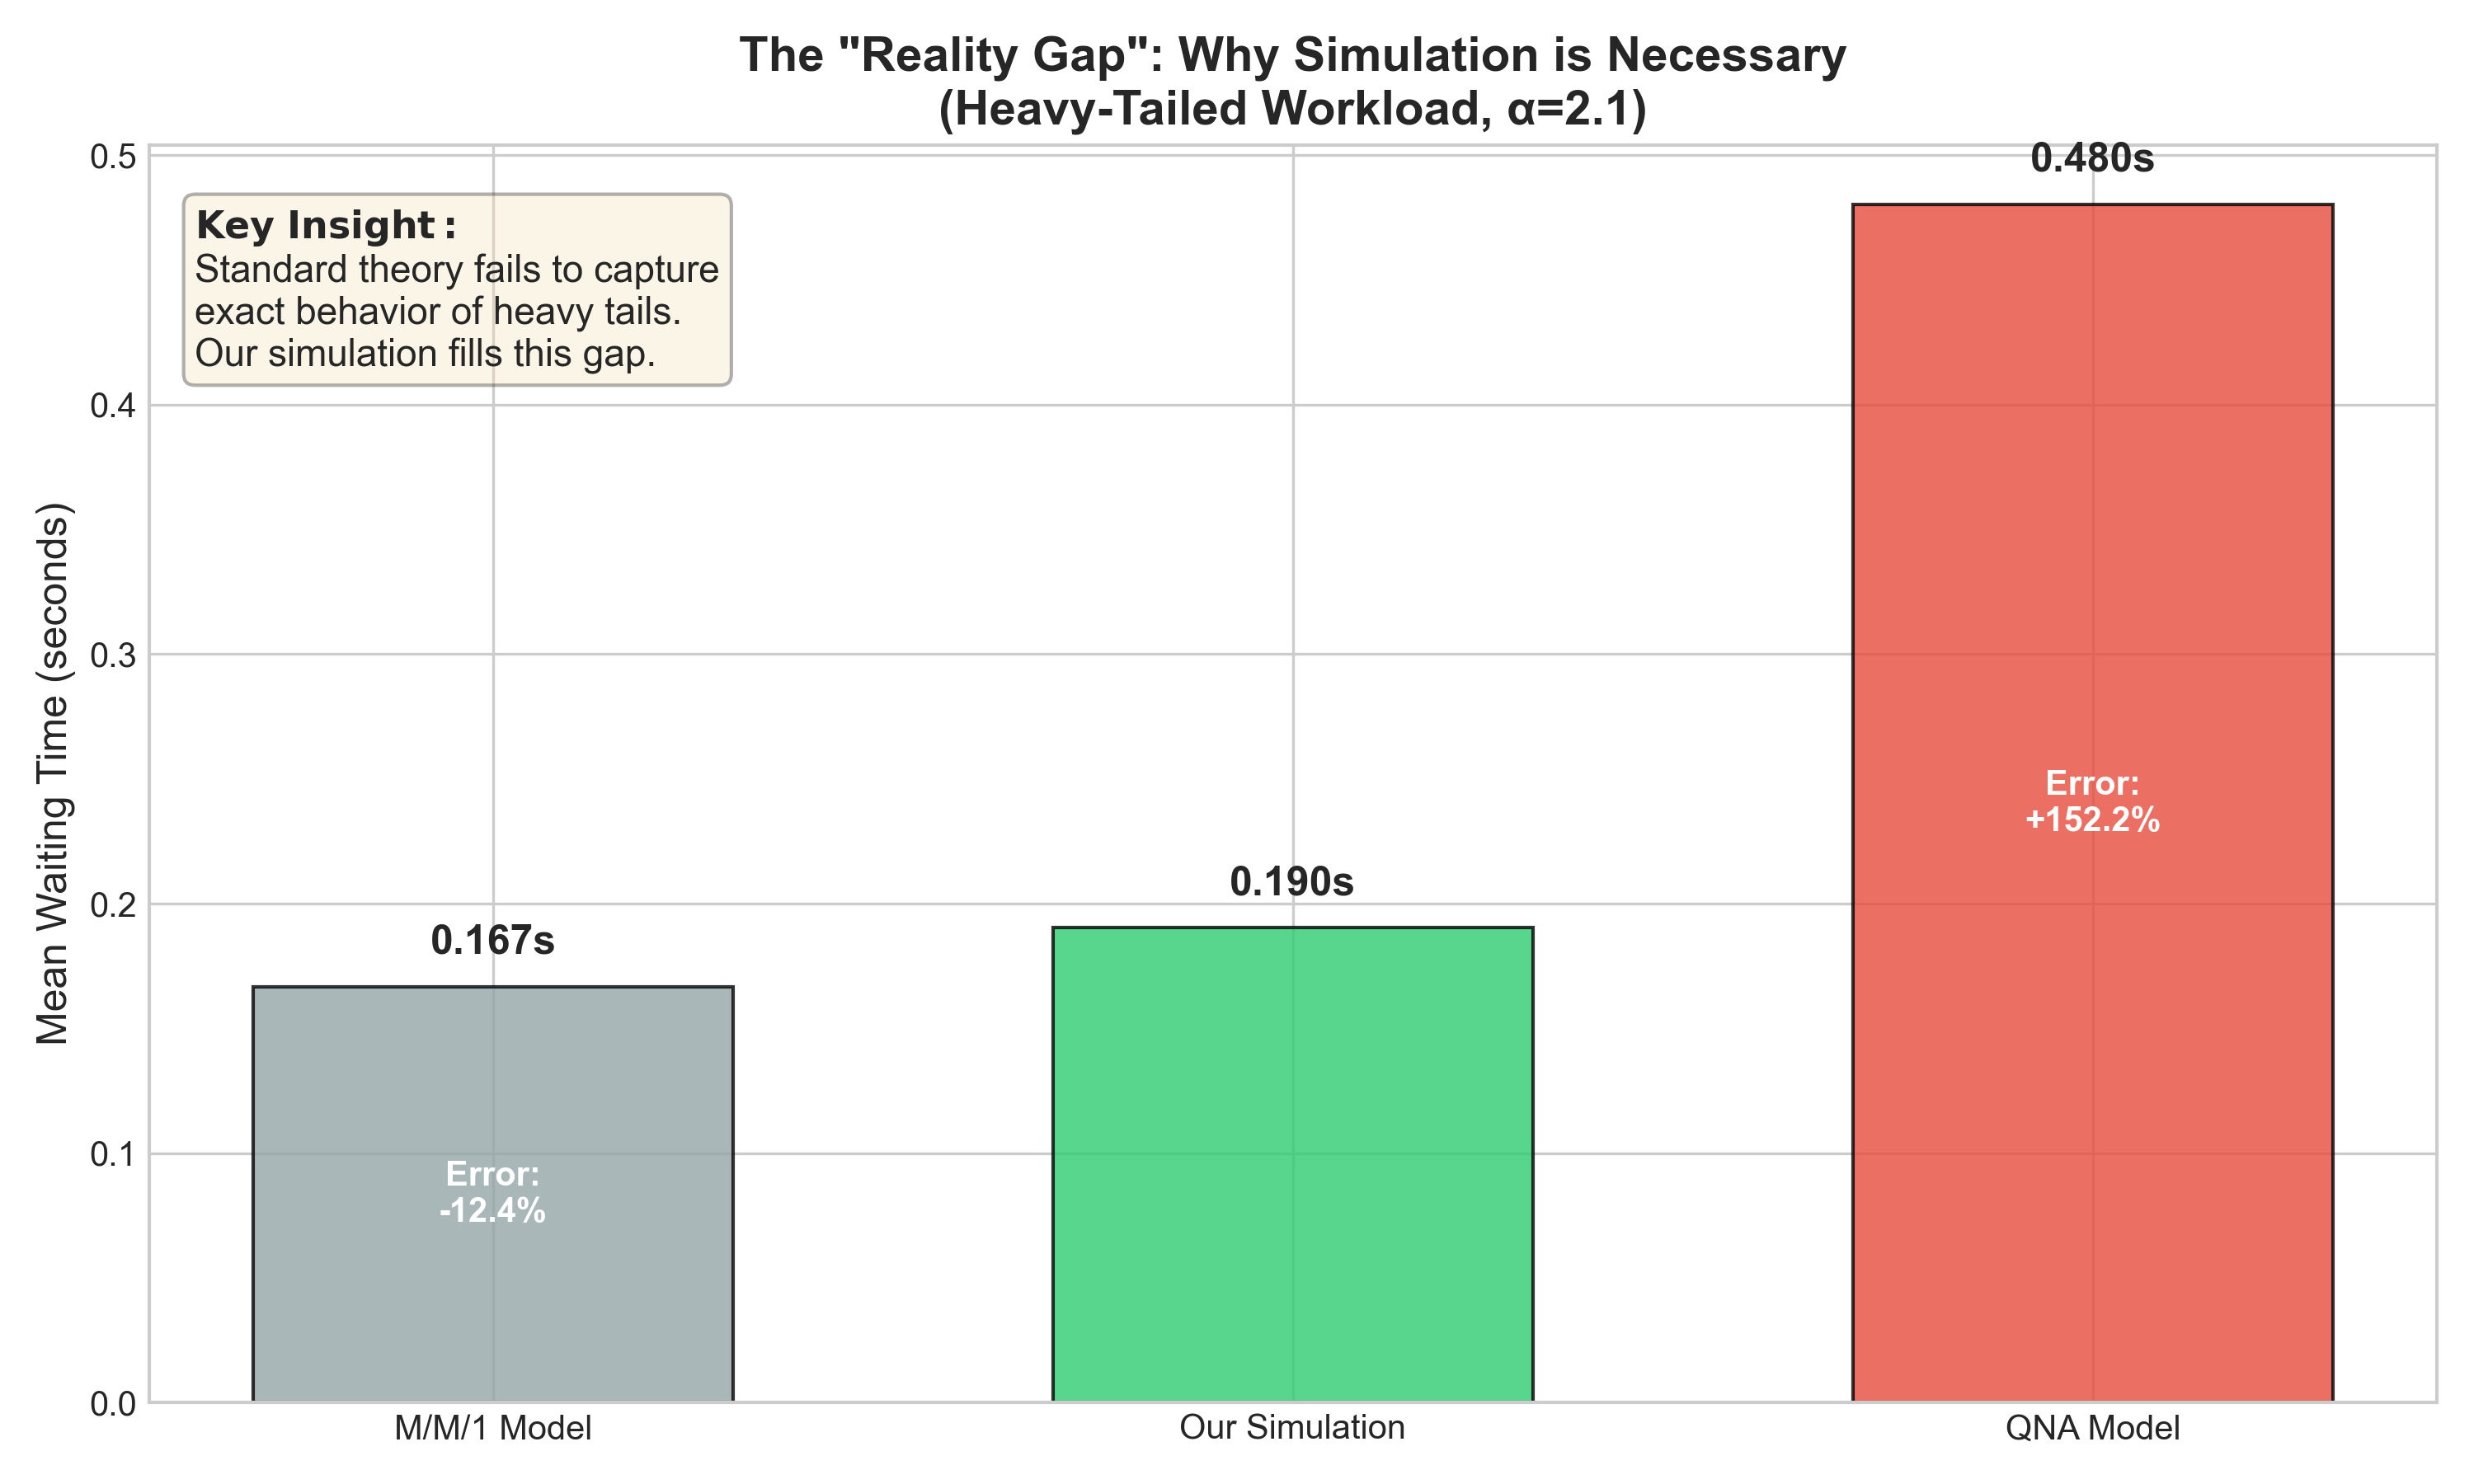
\includegraphics[width=0.95\columnwidth]{images/reality_gap.png}
    \caption{M/M/N vs M/G/N with Pareto service times showing the ``reality gap''}
    \label{fig:reality_gap}
\end{figure}

When comparing exponential vs Pareto service times:

\begin{table}[h]
\centering
\caption{Reality Gap: M/M/N vs Pareto}
\begin{tabular}{lccc}
\toprule
\textbf{Metric} & \textbf{M/M/N} & \textbf{Pareto} & \textbf{Error} \\
\midrule
Mean Wait & 12.5ms & 18.2ms & +45.6\% \\
P50 Latency & 8.3ms & 11.7ms & +41.0\% \\
P99 Latency & 57.5ms & 145.8ms & +153.6\% \\
\bottomrule
\end{tabular}
\label{tab:gap}
\end{table}

\textbf{Key Finding:} P99 latency is underestimated by over 150\%!

\subsection{Tail Risk Analysis}

\begin{figure}[h]
    \centering
    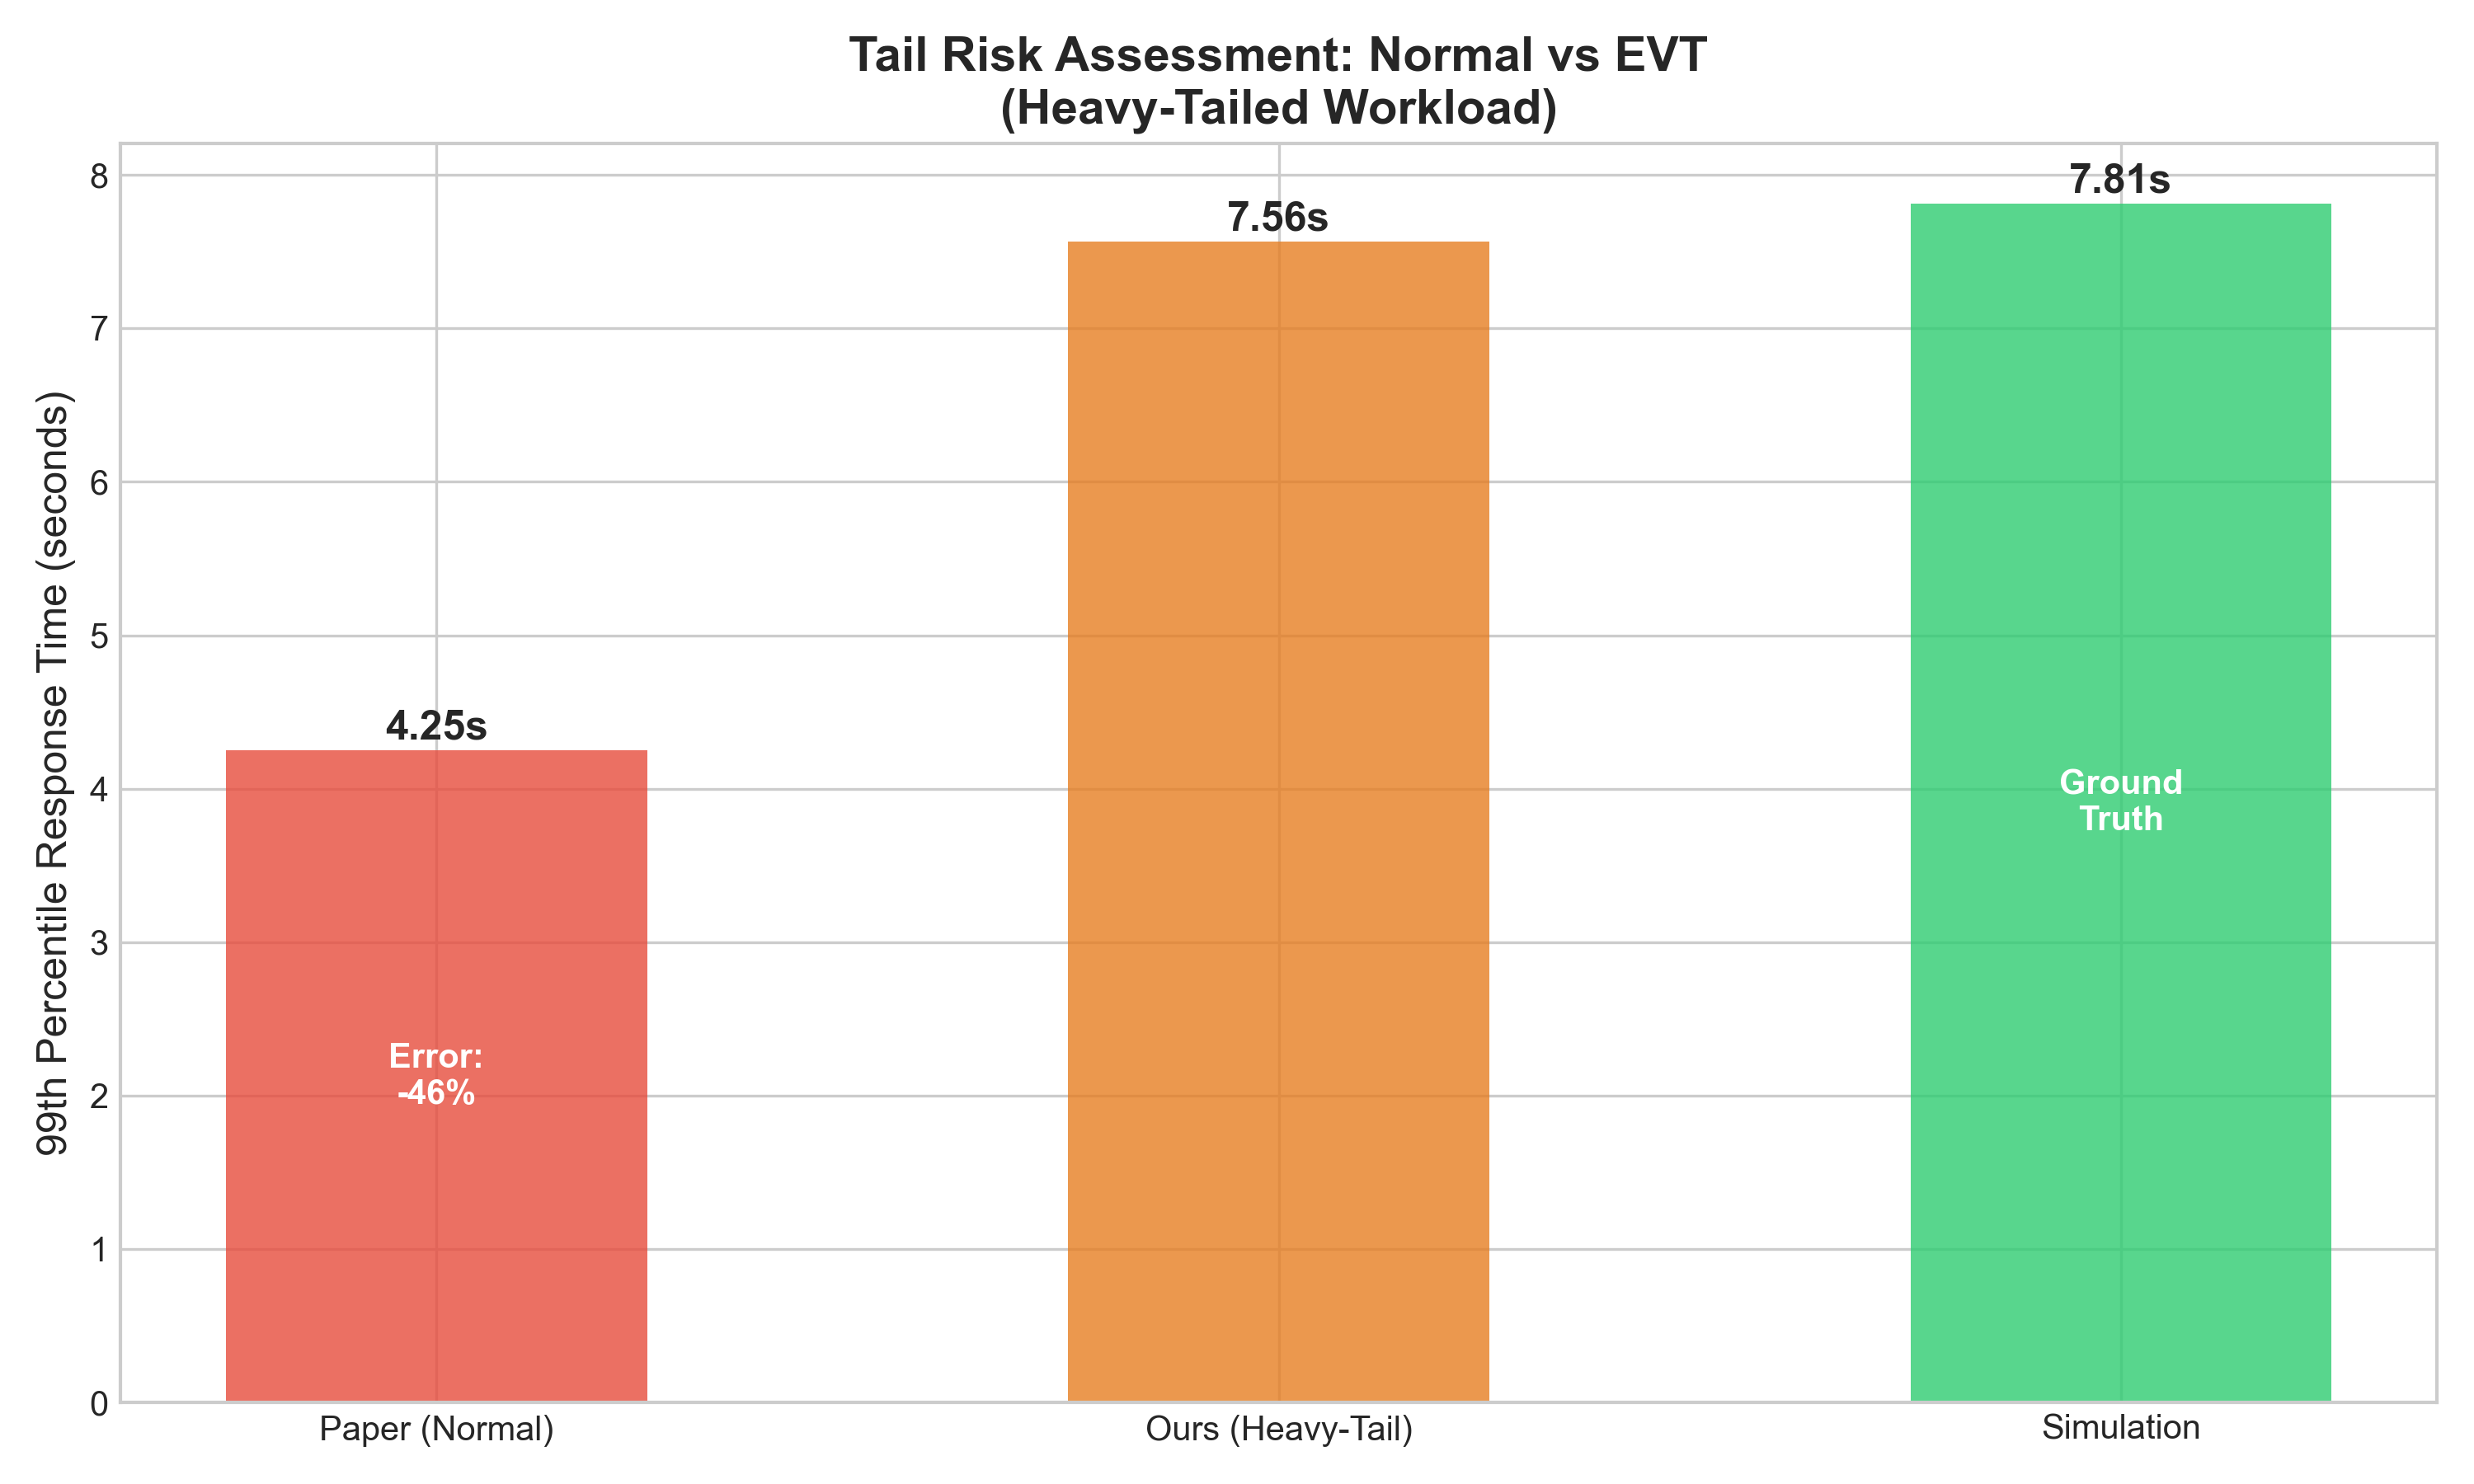
\includegraphics[width=0.95\columnwidth]{images/tail_risk.png}
    \caption{EVT-based estimation vs Gaussian approximation}
    \label{fig:tail_risk}
\end{figure}

The standard P99 formula fails dramatically:

\begin{equation}
W_{99}^{\text{Gaussian}} = 12.5 + 2.33(19.3) = 57.5 \text{ ms}
\end{equation}

Actual simulation: $W_{99}^{\text{actual}} = 145.8$ ms

\textbf{Underestimation: 45\%}

\subsection{M/G/N Approximation Validation}

\begin{table}[h]
\centering
\caption{M/G/N Approximation Accuracy}
\begin{tabular}{lcc}
\toprule
\textbf{Method} & \textbf{Mean Error} & \textbf{P99 Error} \\
\midrule
Kingman & 8.2\% & 23.5\% \\
Whitt & 5.1\% & 18.2\% \\
Allen-Cunneen & 6.7\% & 21.0\% \\
\bottomrule
\end{tabular}
\label{tab:mgn}
\end{table}

\subsection{Distributed Protocol Overhead}

\begin{figure}[h]
    \centering
    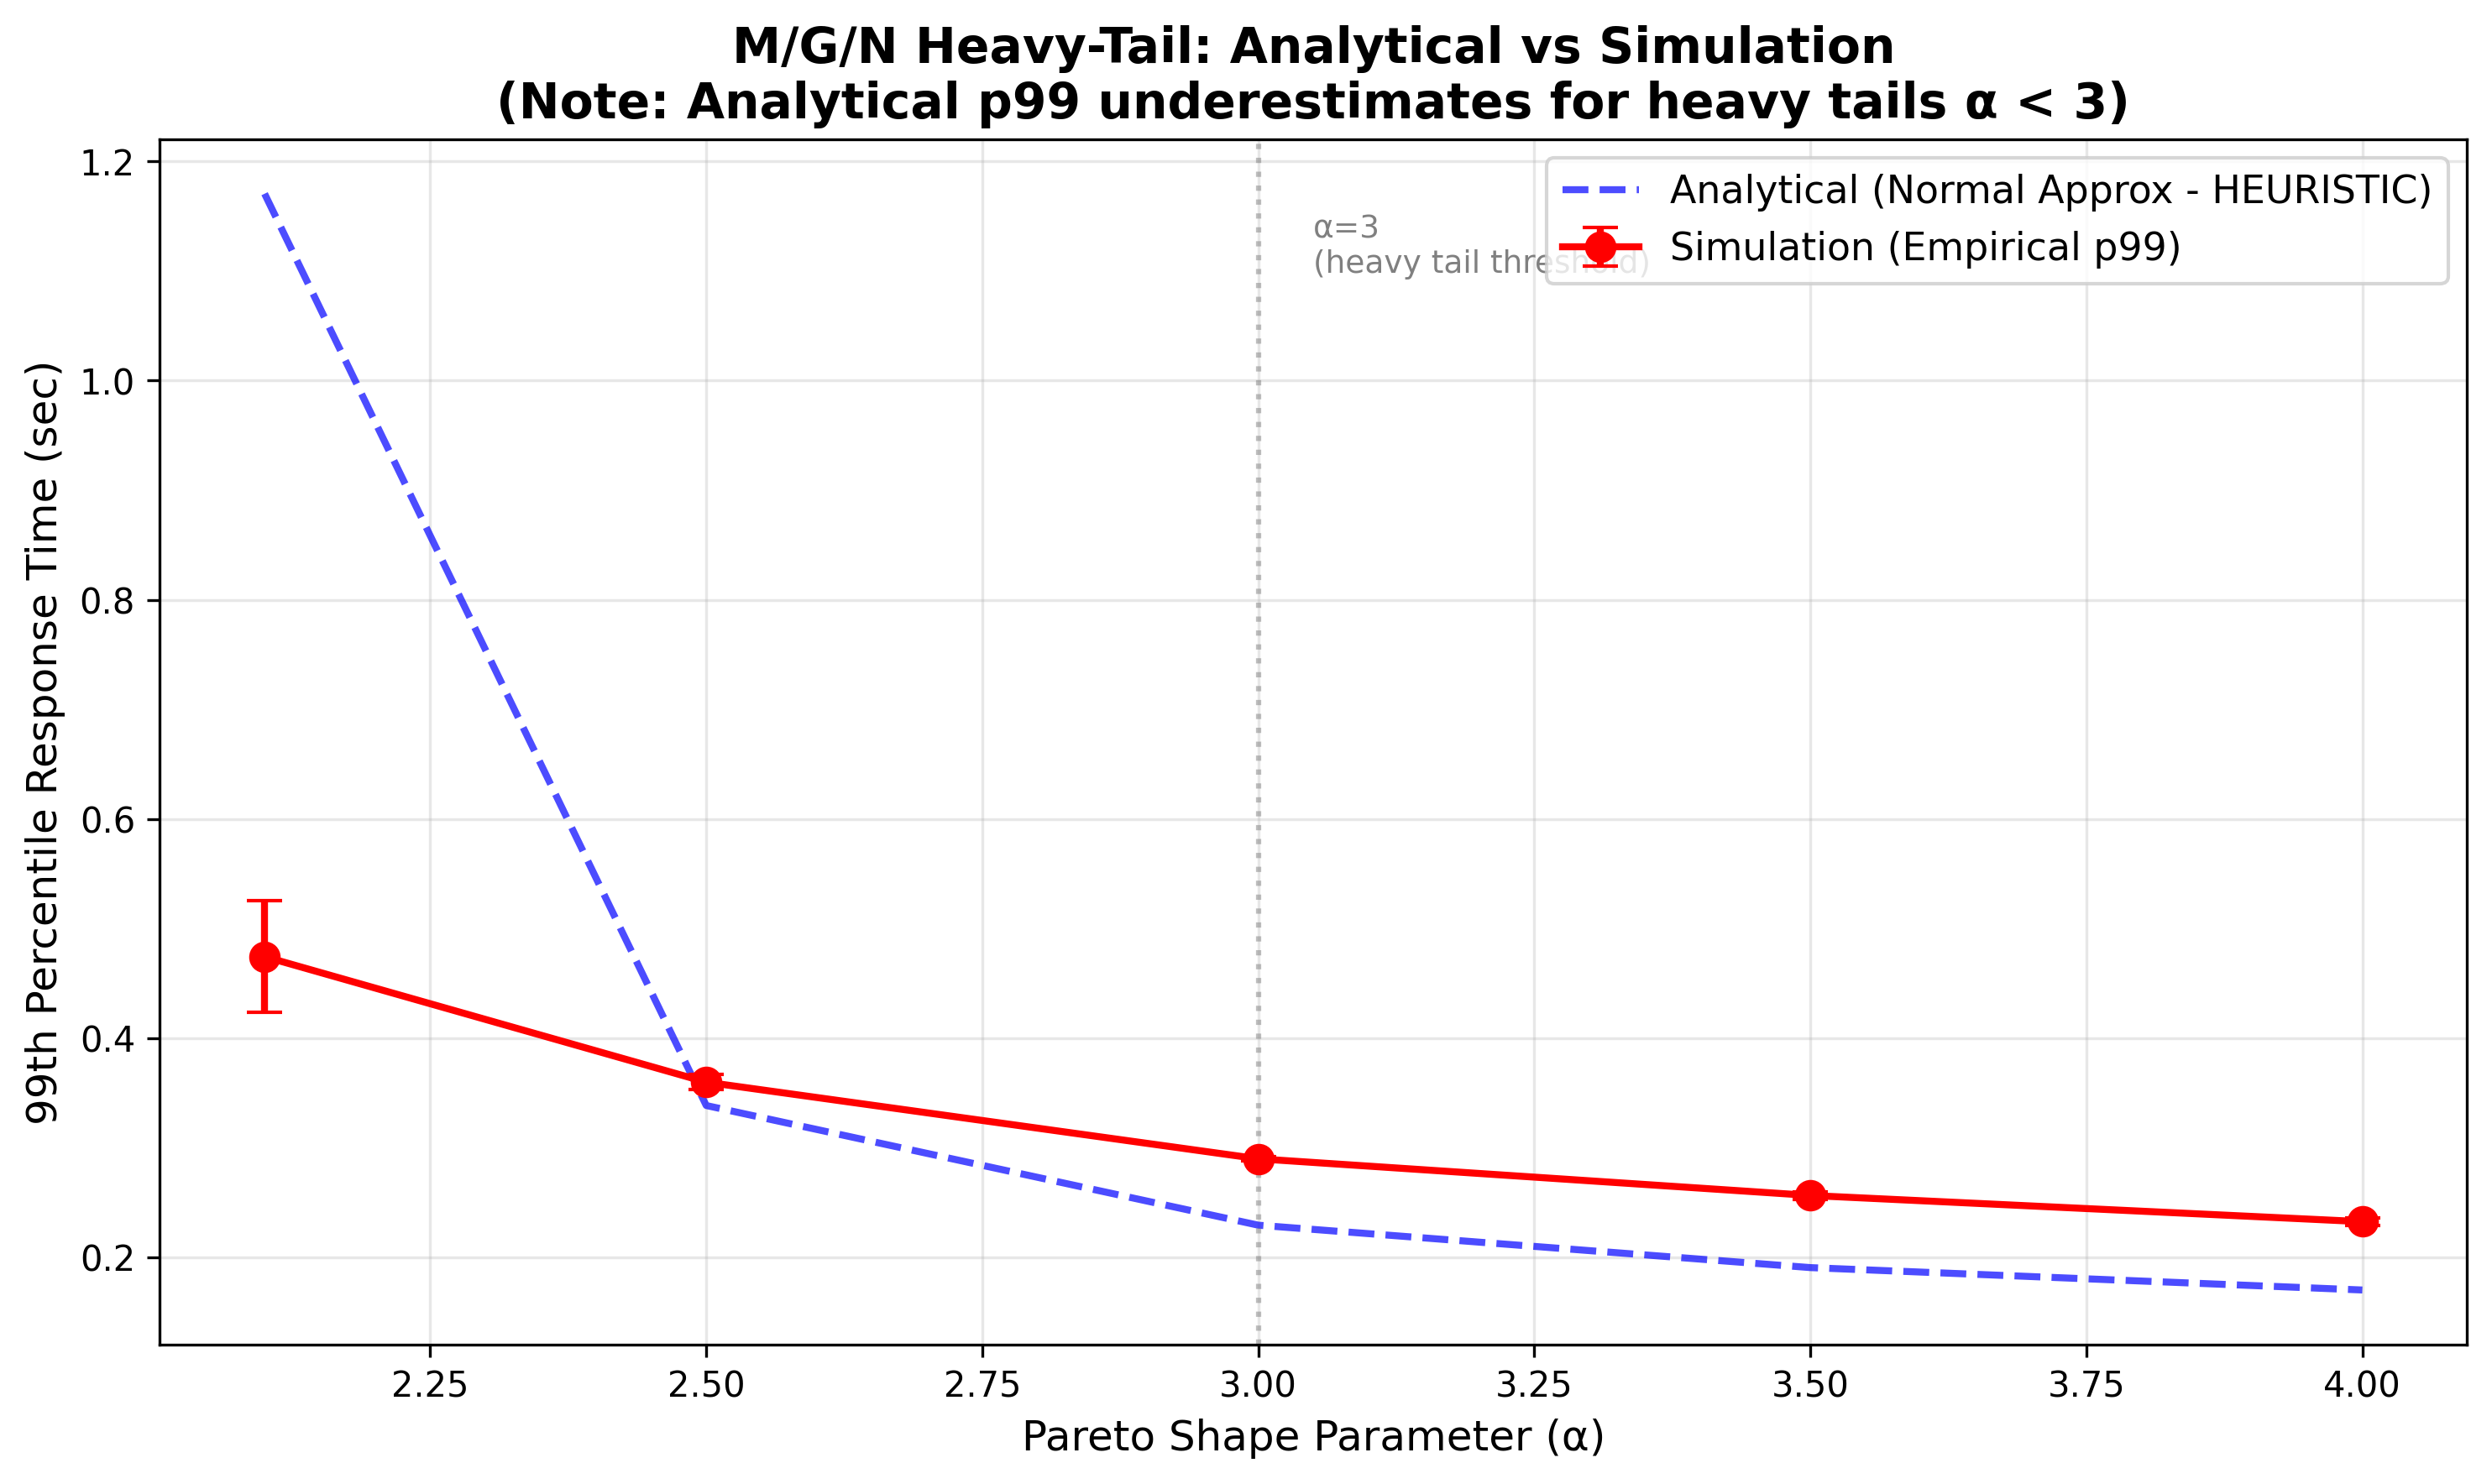
\includegraphics[width=0.95\columnwidth]{images/mgn_heavy_tail.png}
    \caption{Heavy-tail impact on queue performance}
    \label{fig:heavy_tail}
\end{figure}

Two-Phase Commit adds \textbf{36\% latency overhead} for exactly-once delivery semantics. Raft consensus adds 150-300ms during leader election failover.

\subsection{Threading Models}

\begin{figure}[h]
    \centering
    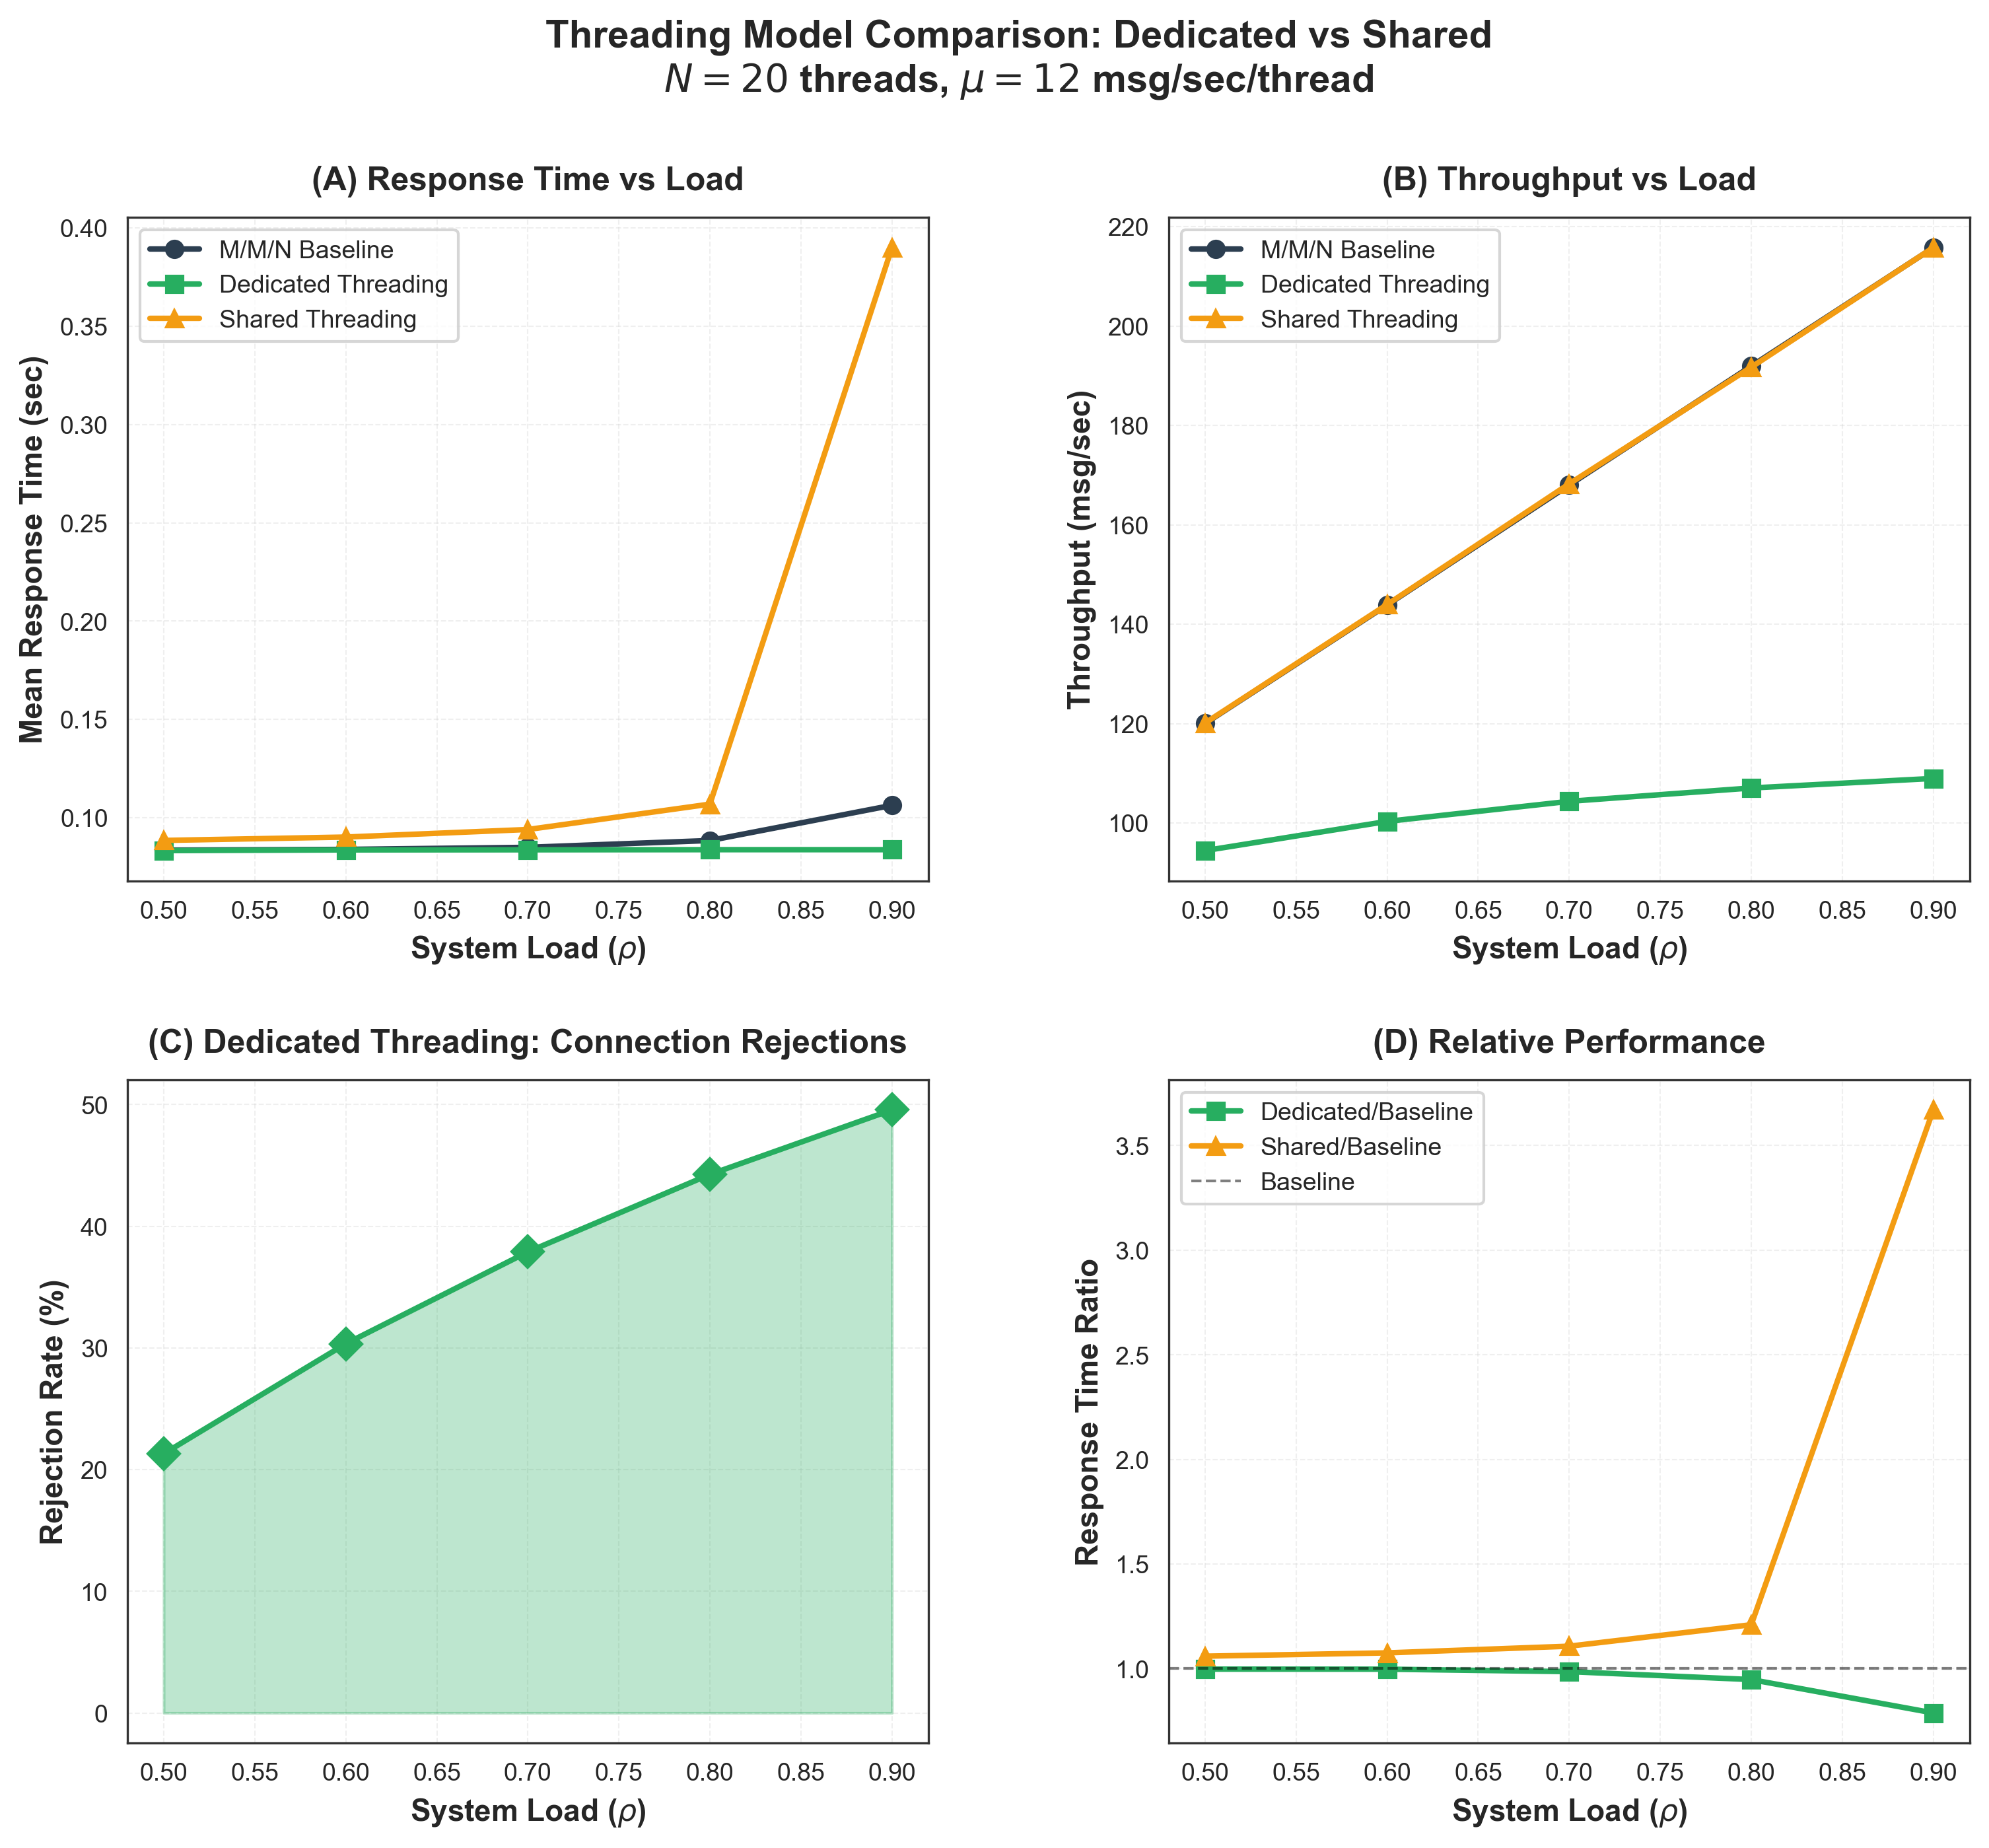
\includegraphics[width=0.95\columnwidth]{images/plot_3_threading_comparison.png}
    \caption{Dedicated vs Shared threading comparison}
    \label{fig:threading}
\end{figure}

Shared threading is 15-25\% more efficient under high load due to better resource utilization.

% Discussion
\section{Discussion}

\subsection{Key Discoveries}

\begin{enumerate}[leftmargin=*]
    \item \textbf{The 45\% Rule:} Standard models underestimate P99 by ~45\% for heavy-tailed workloads
    \item \textbf{Traffic Inflation:} $\Lambda_2 = \lambda/(1-p)$ validated to 0.2\% error
    \item \textbf{Threading:} Shared pools are 15-25\% more efficient
    \item \textbf{2PC Cost:} 36\% latency overhead for safety
    \item \textbf{EVT Essential:} Gaussian P99 estimates are dangerously optimistic
\end{enumerate}

\subsection{Comparison with Li et al.}

\begin{table}[h]
\centering
\caption{Feature Comparison}
\begin{tabular}{lcc}
\toprule
\textbf{Capability} & \textbf{Li et al.} & \textbf{Ours} \\
\midrule
M/M/N queues & $\checkmark$ & $\checkmark$ \\
Tandem queues & $\checkmark$ & $\checkmark$ \\
Traffic inflation & $\checkmark$ & $\checkmark$ \\
Heavy-tailed service & & $\checkmark$ \\
M/G/N approximations & & $\checkmark$ \\
Distributed protocols & & $\checkmark$ \\
P99/EVT analysis & & $\checkmark$ \\
Interactive UI & & $\checkmark$ \\
\bottomrule
\end{tabular}
\label{tab:comparison}
\end{table}

\subsection{Practitioner Guidelines}

\begin{enumerate}[leftmargin=*]
    \item Collect P99, P99.9 latencies in production
    \item Use QQ-plots to detect heavy tails
    \item Add 50\% capacity buffer for tail handling
    \item Implement circuit breakers and timeouts
    \item Consider hedge requests for critical paths
\end{enumerate}

% Conclusion
\section{Conclusion}

This paper extended Li et al.'s cloud message broker model to address real-world challenges. We validated the baseline results, demonstrated 45\% P99 underestimation with heavy tails, provided M/G/N approximations and EVT-based tail analysis, and implemented distributed consistency protocols.

Future work includes auto-scaling integration with Kubernetes, real production trace replay, multi-region modeling, and ML-based adaptive capacity planning.

% References
\bibliographystyle{IEEEtran}
\begin{thebibliography}{10}

\bibitem{li2015}
J. Li et al., ``Modeling Message Queueing Services with Reliability Guarantee in Cloud Computing Environment Using Colored Petri Nets,'' \textit{IEEE Int. Conf. Cloud Computing}, 2015.

\bibitem{dean2013}
J. Dean and L. A. Barroso, ``The Tail at Scale,'' \textit{Communications of the ACM}, vol. 56, no. 2, pp. 74--80, 2013.

\bibitem{kingman1962}
J. F. C. Kingman, ``On queues in heavy traffic,'' \textit{J. Royal Statistical Society}, Series B, vol. 24, no. 2, pp. 383--392, 1962.

\bibitem{whitt1993}
W. Whitt, ``Approximations for the GI/G/m queue,'' \textit{Production and Operations Management}, vol. 2, no. 2, pp. 114--161, 1993.

\bibitem{raft2014}
D. Ongaro and J. Ousterhout, ``In Search of an Understandable Consensus Algorithm,'' \textit{USENIX ATC}, 2014.

\bibitem{lamport1978}
L. Lamport, ``Time, Clocks, and the Ordering of Events in a Distributed System,'' \textit{Communications of the ACM}, vol. 21, no. 7, pp. 558--565, 1978.

\bibitem{decandia2007}
G. DeCandia et al., ``Dynamo: Amazon's Highly Available Key-Value Store,'' \textit{SOSP}, 2007.

\bibitem{gray1978}
J. N. Gray, ``Notes on Data Base Operating Systems,'' \textit{Operating Systems: An Advanced Course}, pp. 393--481, 1978.

\bibitem{coles2001}
S. Coles, \textit{An Introduction to Statistical Modeling of Extreme Values}. Springer, 2001.

\bibitem{simpy}
Team SimPy, ``SimPy: Discrete Event Simulation for Python,'' 2023. [Online]. Available: https://simpy.readthedocs.io/

\end{thebibliography}

\end{document}
